\subsubsection{Entidades}
A continuación, en las figuras \ref{DCERed}, \ref{DE1}, \ref{DE2} y \ref{DE3}, se mostrará más a detalle el contenido que tiene cada uno de los paquetes ilustrados anteriormente. Como primera parte, se muestran las clases que están dentro del paquete \\ `com.example.PruebaCRUD.Entities`. En este diagrama se muestran las relaciones internas entre las clases dentro del paquete ya mencionado.

\begin{figure}[htbp!]
	\begin{center}
		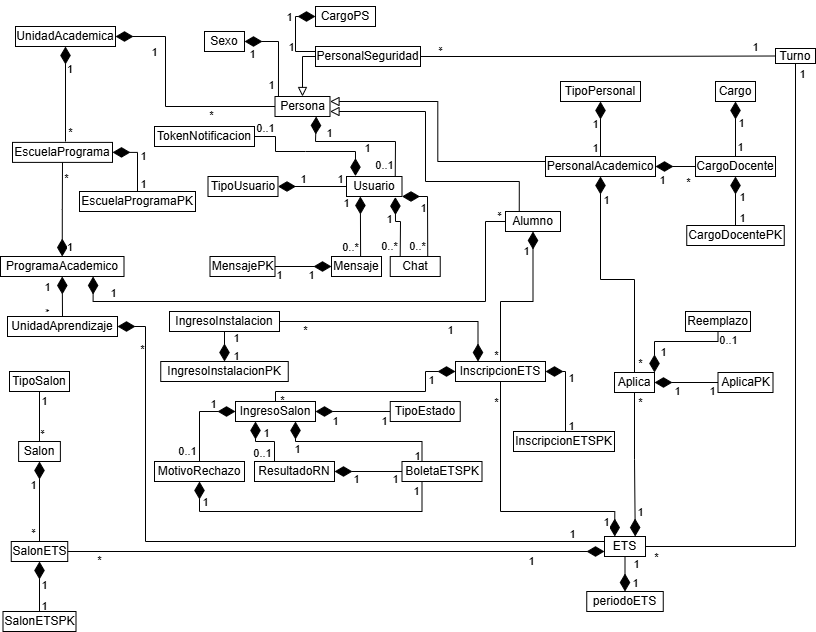
\includegraphics[width=0.8\textwidth]{Clases/DCE Reducido.png}
		\caption{Diagrama de clases general de las entidades del servidor.}
		\label{fig:DCERed}
	\end{center}
\end{figure}

 En este primer diagrama, las clases se muestran sin sus propiedades para una mejor visualización, sin embargo, en las imágenes posteriores se detalla más a profundidad las propiedades de cada una de estas clases.

\newpage

\begin{figure}[htbp!]
	\begin{center}
		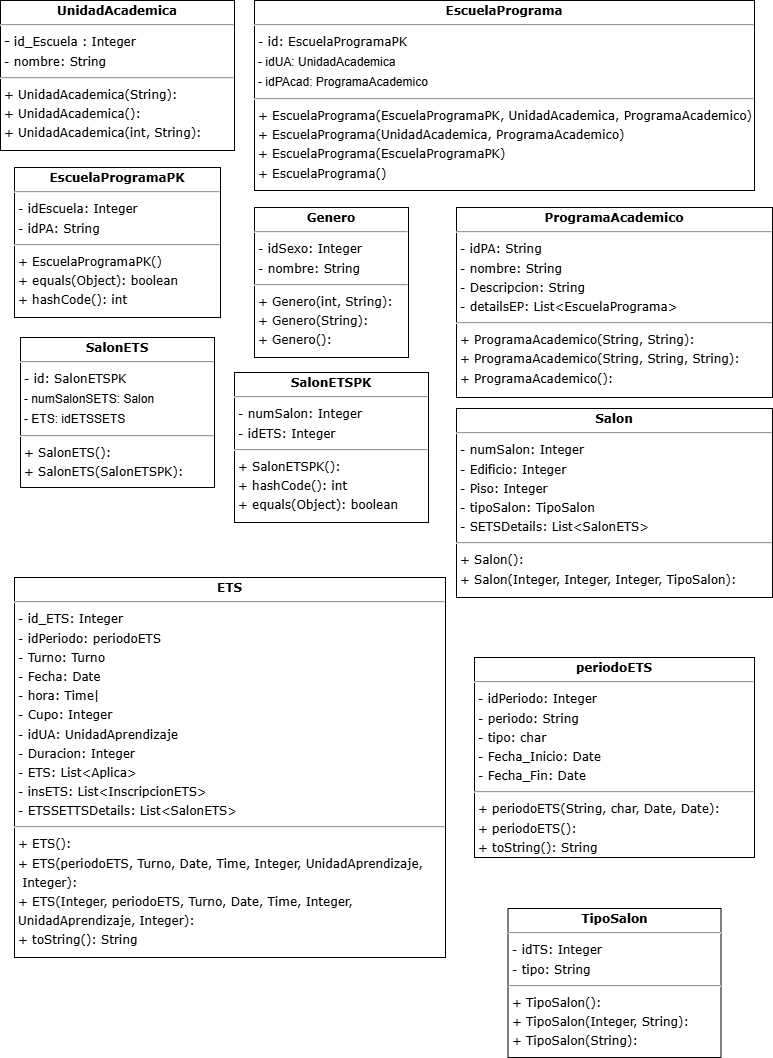
\includegraphics[width=0.8\textwidth]{Clases/EntidadesP1.png}
		\caption{Diagrama de clases de las entidades del servidor parte 1.}
		\label{fig:DE1}
	\end{center}
\end{figure}


\begin{figure}[htbp!]
	\begin{center}
		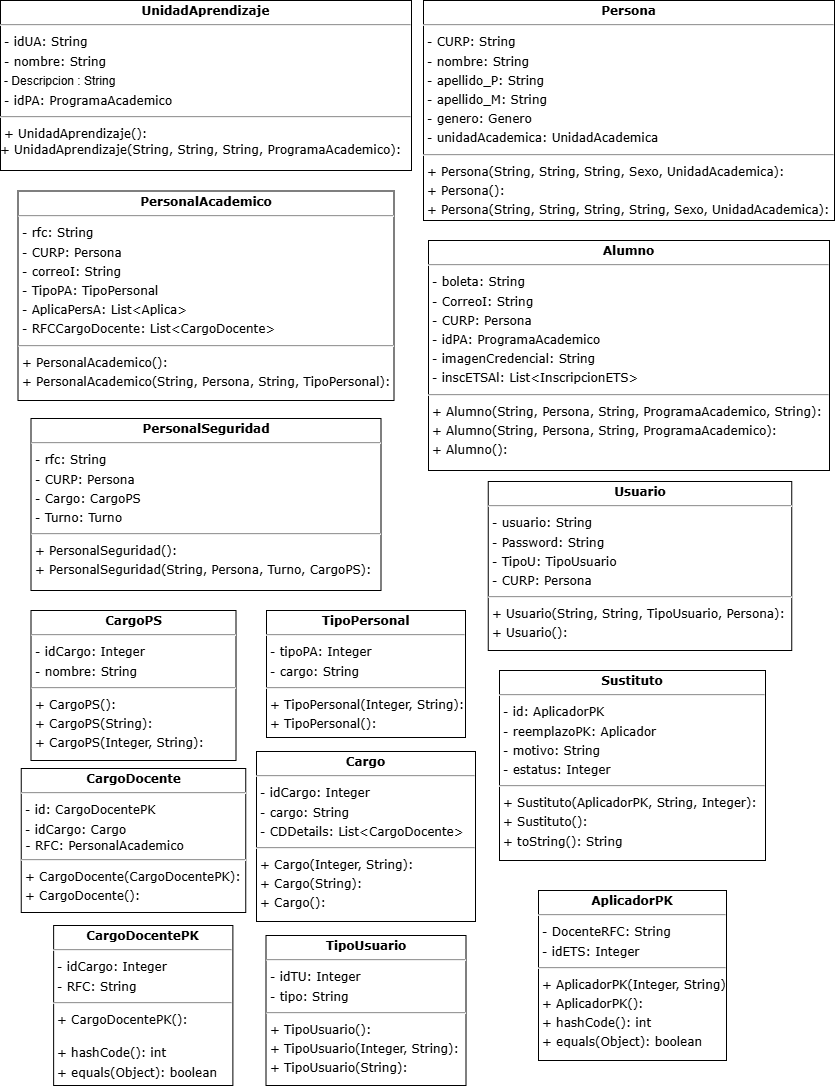
\includegraphics[width=0.8\textwidth]{Clases/EntidadesP2.png}
		\caption{Diagrama de clases de las entidades del servidor parte 2.}
		\label{fig:DE2}
	\end{center}
\end{figure}


\begin{figure}[htbp!]
	\begin{center}
		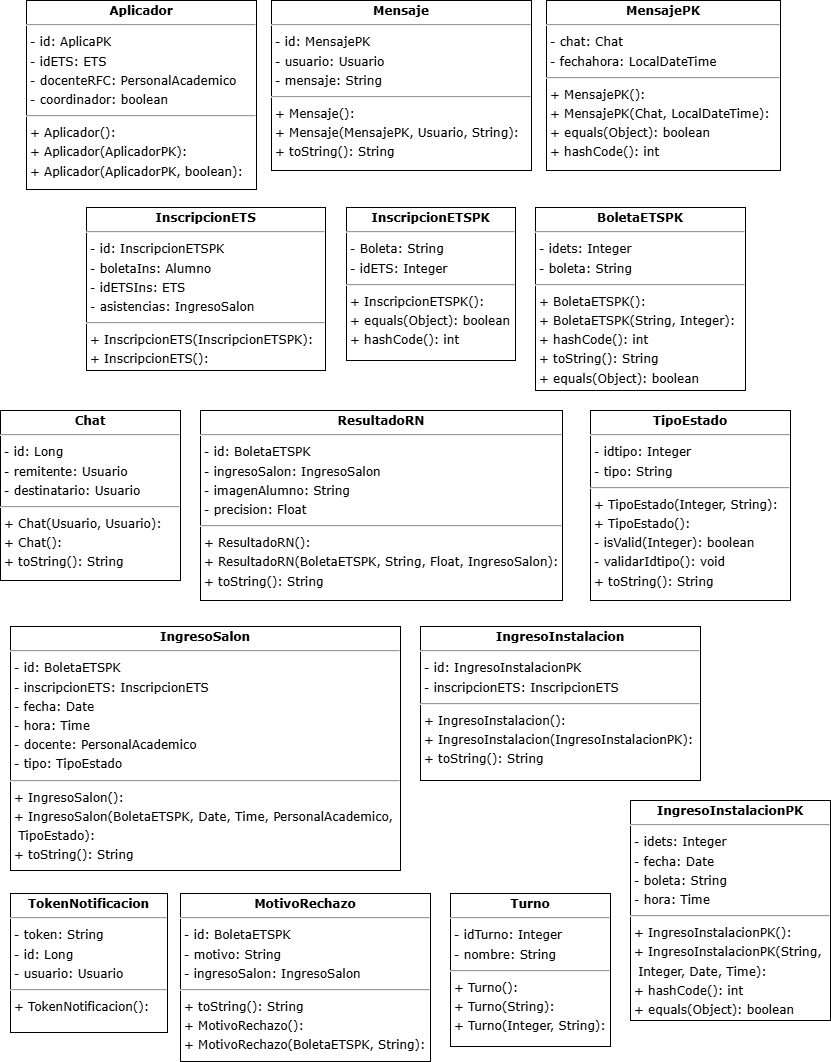
\includegraphics[width=0.8\textwidth]{Clases/EntidadesP3.png}
		\caption{Diagrama de clases de las entidades del servidor parte 3.}
		\label{fig:DE3}
	\end{center}
\end{figure}

\newpage